\chapter{Arduino sensor specification and implementation}\label{cap:implementacion}

\section{Introduction}
There are infinitely many ways of implementing sensors in a computer system. Internet of things is slowly becoming a topic that people interested in technology are talking about. For our particular case, we will be using an Arduino MEGA 2560 board.

\begin{figure}[H]
    \centering
    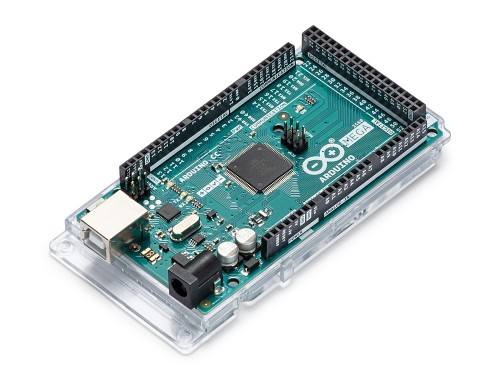
\includegraphics[width=0.5\textwidth]{fig/mega2560.jpg}
    \caption{Arduino MEGA 2560 board}
    \label{fig:mega2560}
\end{figure}



\section{Sensors' implementation}
Let's take a look at some of the options that the different sensors offer. In this section we will specify some sensors in order to understand what these components are capable of, then, we will implement the two of them that are considered to be more crucial in harvesting, since those are the ones that we are interested in for this prototype. 

We know we will be working with an Arduino MEGA 2560 board, but it goes without saying, we will also need some more components. 

\subsection{FC-28 Soil Moisture Sensor}
Soil moisture sensor is likely the main sensor when harvesting is concerned as it helps farmers manage their irrigation systems more efficiently. This won't only save water but will also increase the quality of the crops since it can control moisture to the milimeter at all diferent plant growth stages. In this section, we are going to be documenting the process of using the sensor FC-28 with our Arduino board.

\subsubsection{How does it work?}
This FC-28 hygrometer module consists of two probes that measure the volumetric content of water. The current passes through the soil, which gives the resistance value between the metallic probes and measures the moisture value. The reason why this works fine is simple: the more water a soil has, the more electricity will be conducted which means less resistance.

\begin{figure}[H]
    \centering
    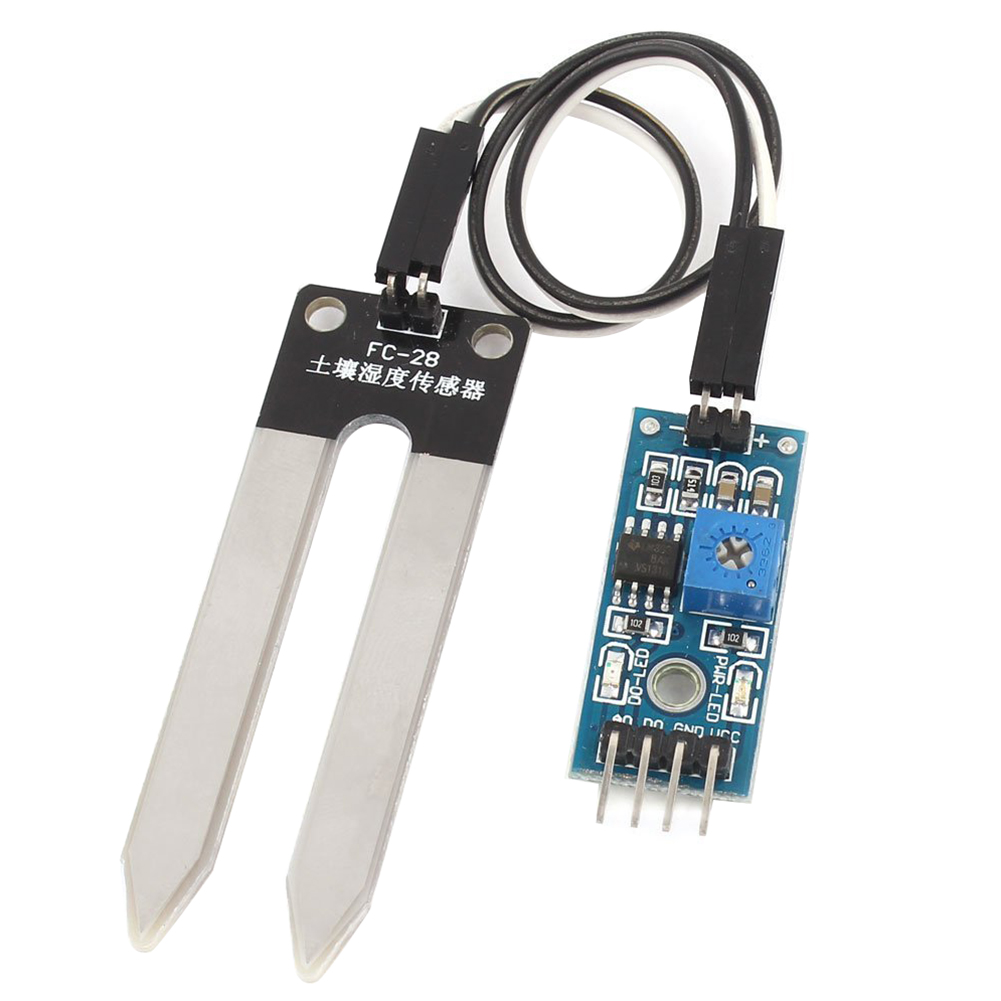
\includegraphics[width=0.35\textwidth]{fig/fc28.jpg}
    \caption{A FC-28 moisture sensor}
    \label{fig:fc28}
\end{figure}

Besides the sensor itself, there is another component that has two LEDs (one for output and another for power), a potentiometer and a LM293 comparator.

\subsubsection{Using the sensor}
The values that the sensor picks up goes from 0 to 1023. Ideally it would show 0 when sunken underwater and 1023 when is only in contact with the air, in other words, when it's not in contact with soil.

Let's implement a small script to understand the behaviour of the sensor. The circuit that we will be using is really simple:
\begin{itemize}
	\item The VCC of the FC-28 goes to 5V of the Arduino
	\item The GND of the FC-28 goes to GND of the Arduino
	\item The pin A0 of the FC-28 goes to the pin A0 of the Arduino
\end{itemize}
Here's a diagram of the circuit.

\begin{figure}[H]
    \centering
    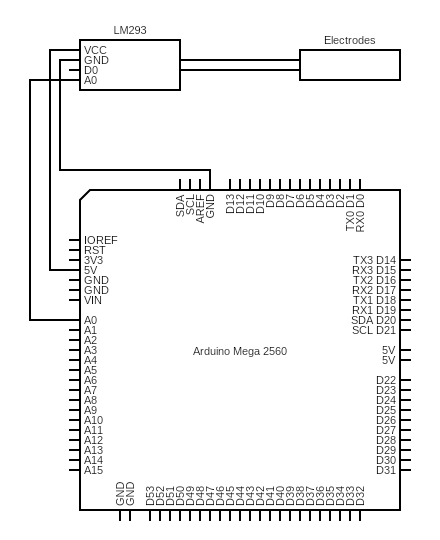
\includegraphics[width=0.5\textwidth]{fig/fc28-scheme-circuit.png}
    \caption{Diagram of the circuit for the FC-28}
    \label{fig:fc28-scheme-circuit}
\end{figure}


This is how circuit should look like once assembled.
	\begin{figure}[H]
		\centering
		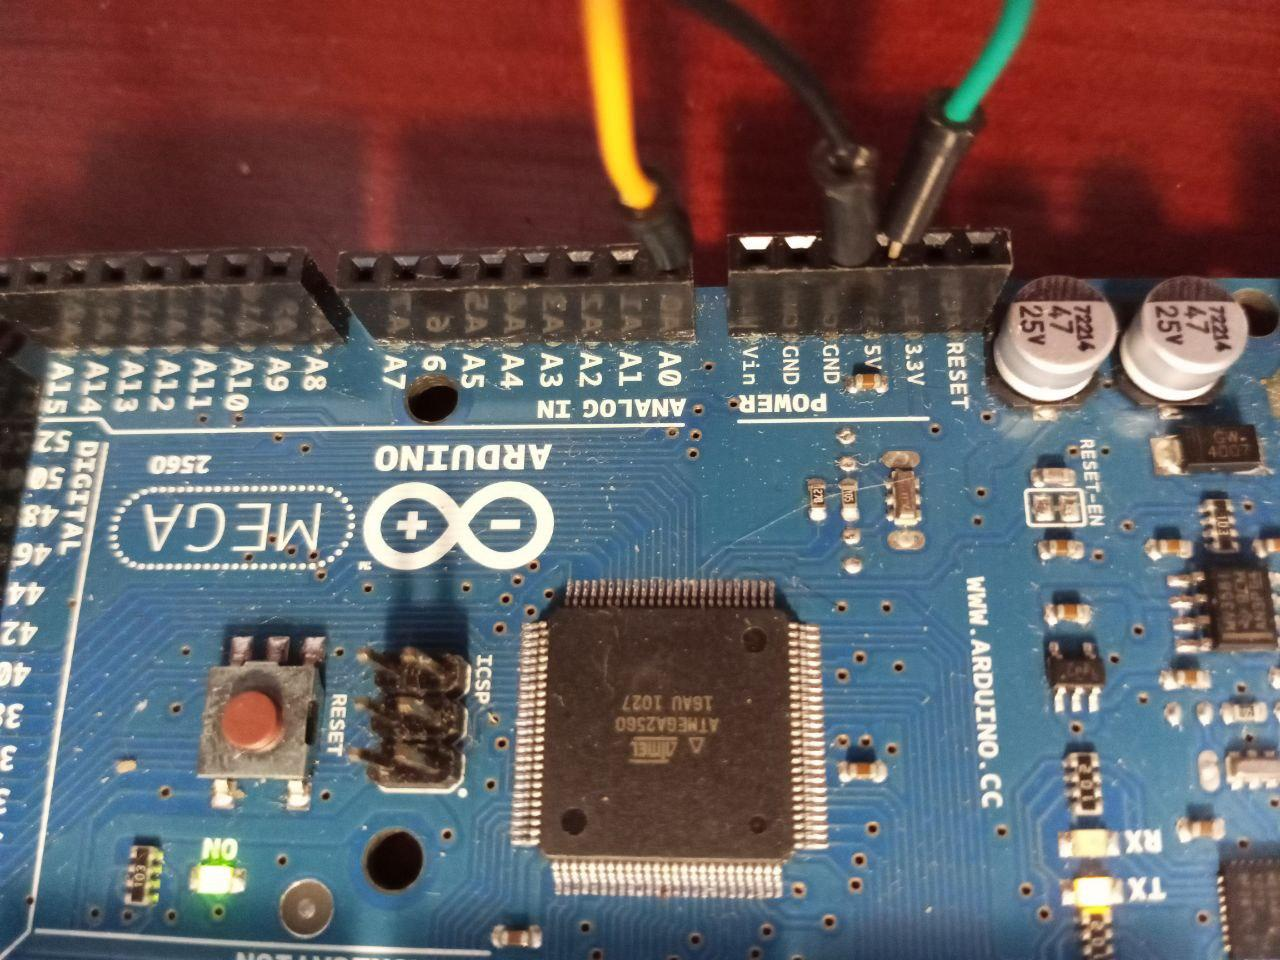
\includegraphics[width=0.35\textwidth]{fig/fc28-circuit1.jpg}
		\caption{Board for FC-28 connections}
	\end{figure}
	\hfill
	\begin{figure}[H]
		\centering
		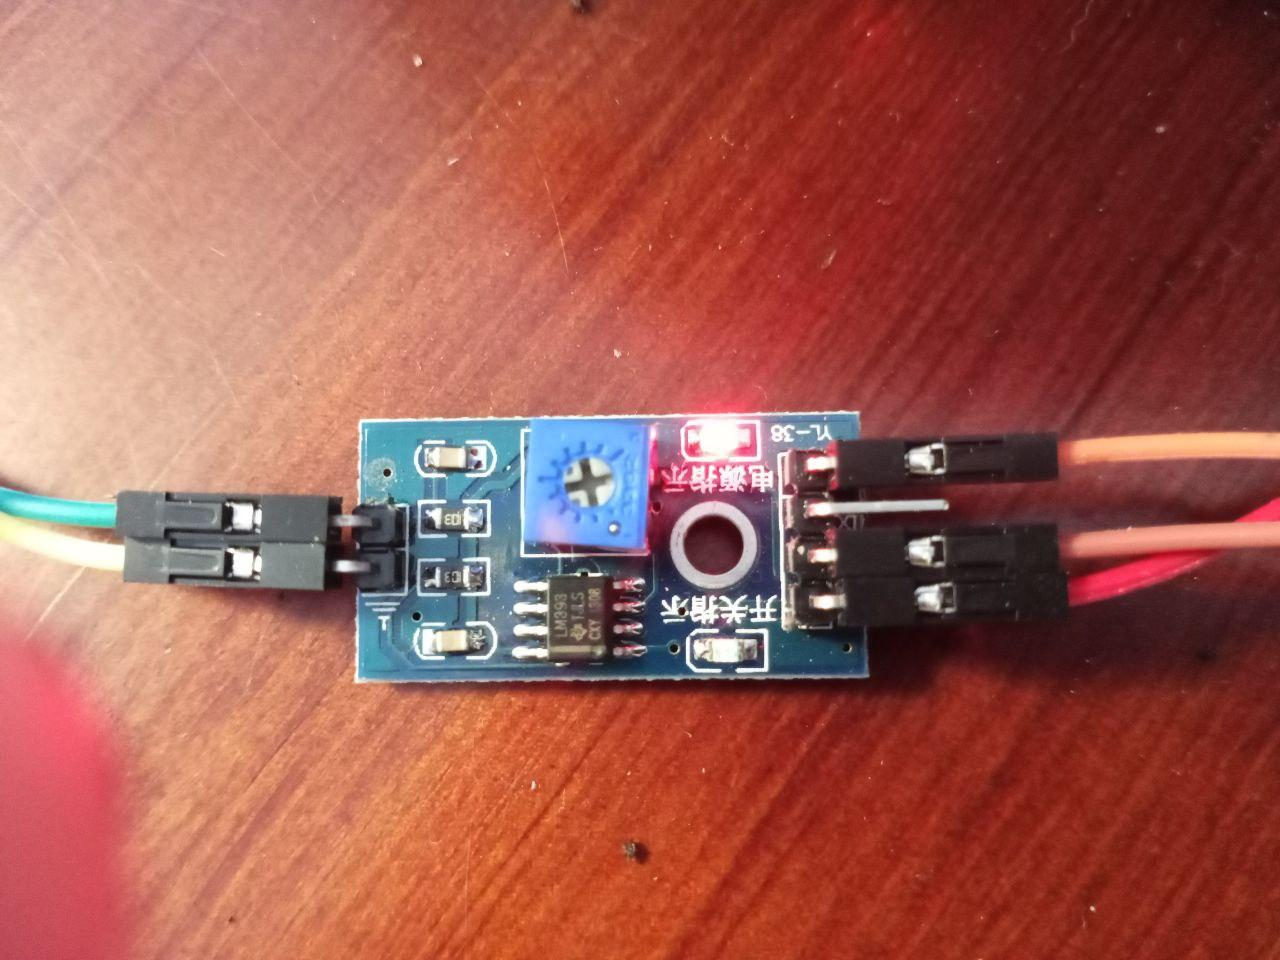
\includegraphics[width=0.35\textwidth]{fig/fc28-circuit2.jpg}
		\caption{LM293 comparator}
	\end{figure}

Now let's take a look at the script that is going to make the sensor work

\lstinputlisting{arduino/fc28.ino}

Since this is the first piece of code introduced in this project, we will use this FC-28 sensor code to explain just a bit of how code is structured in Arduino and why it has to be this way. For the rest of the sensors, the code is more less similar so the explanation of the code will be more straight-forward.

\vspace{7mm}
\textbf{Introduction to Arduino program structure}

Before we step in, it catchs our eye that there are two well distingued functions: void setup() and void loop(). There two functions are \textbf{mandatory} in Arduino. If we try to execute code that lacks any of them, we'll get an error. See an example below.

(error x faltar una funcion mandatory)

There is actually a really simple reason why. In a tipical C/C++ program, a main function is needed. That is the function that will be called first and at the same time, the function where the rest of functions will be called.

In Arduino there is no main, so instead, we have these two. Now another question might be crossing our minds, which is the purpose of each function?

\begin{itemize}
	\item \textbf{setup().} The code inside this function will be execute exactly once at the very beginning of the execution. Some examples of instructions that typically go inside setup() are pinMode, Serial.begin, initialisation of libraries that might be included, etc.
	\item \textbf{loop().} This is the main function of the program, all the code written here will be executed again and again as long as the Arduino board is enabled, of course that is why is the loop function. It goes from the very first line until the last one secuentially, skipping inmediately to the line 1 again. It'll go like this forever as long as the board is provided with electrical supply.
\end{itemize}

\newpage

\textbf{FC-28 code explanation}

Enough of Arduino syntax, let's jump in the FC-28 code. In line 1 we are defining the Arduino pin that will read the data gathered from the sensor, for this particular case we have decided the pin will be A0.

We jump now inside of setup() and we find Serial.begin(9600);. If the reader has had the chance to read some Arduino scripts, that line will surely ring a bell, but why do we need to use if? What happens if you change 9600 to another value? What does 9600 even mean?

Serial.begin() establishes a serial communication between our Arduino board and another device, in this case the other device is my laptop via USB cable. Once that communication has been established the devices can exchange information using a serial protocol.

This explains as well why this instruction is written in setup() function: we know that will only be executed once and we will only need to establish serial communication once.

In regards to the number 9600, we are talking here about the \textbf{baud rate}. This is the data rate in bits per second for serial data transmission \cite{baud}. The default value for Arduino is 9600.

Let's go now to line 8, already inside of the infinite loop. We see a variable is declared there, humidity, it is reading from the sensorPin we've defined before. The reason why we are using analogRead instead of digital is because digital values are only 1 or 0. So if we were to use digitalRead(), it will just return the rounded the analog value. It is more suitable for gathering sensor data to use analogRead().

Good. So now we have a variable humidity that stores the analog value from the FC-28 sensor. Let's print it. As it was mentioned before, FC-28 value range goes from  to 1023, so 500 sounds like a reasonable mid point. As a first approach, we will set 500 as the breakpoint for determining whether it is very wet or very dry with a simple conditional.

We will make this code a bit more especific in the implementation, but in this section we are mainly interested in understanding the sensor behaviour.

This pretty much sums up the code of the FC-28 sensor as well as the main structure of an Arduino program.

\subsubsection{Example: two cases scenarios for this code.}

After understanding a bit how the FC-28 sensor works. Let's see a real life practical example of how this actually works.

\textbf{First case scenario: a really dry Erica} \\
For our particular example we have this beautiful Erica plant. It is planted in a simple plastic pot, and at this precise moment it is absolutely dry.

\begin{figure}[H]
    \centering
    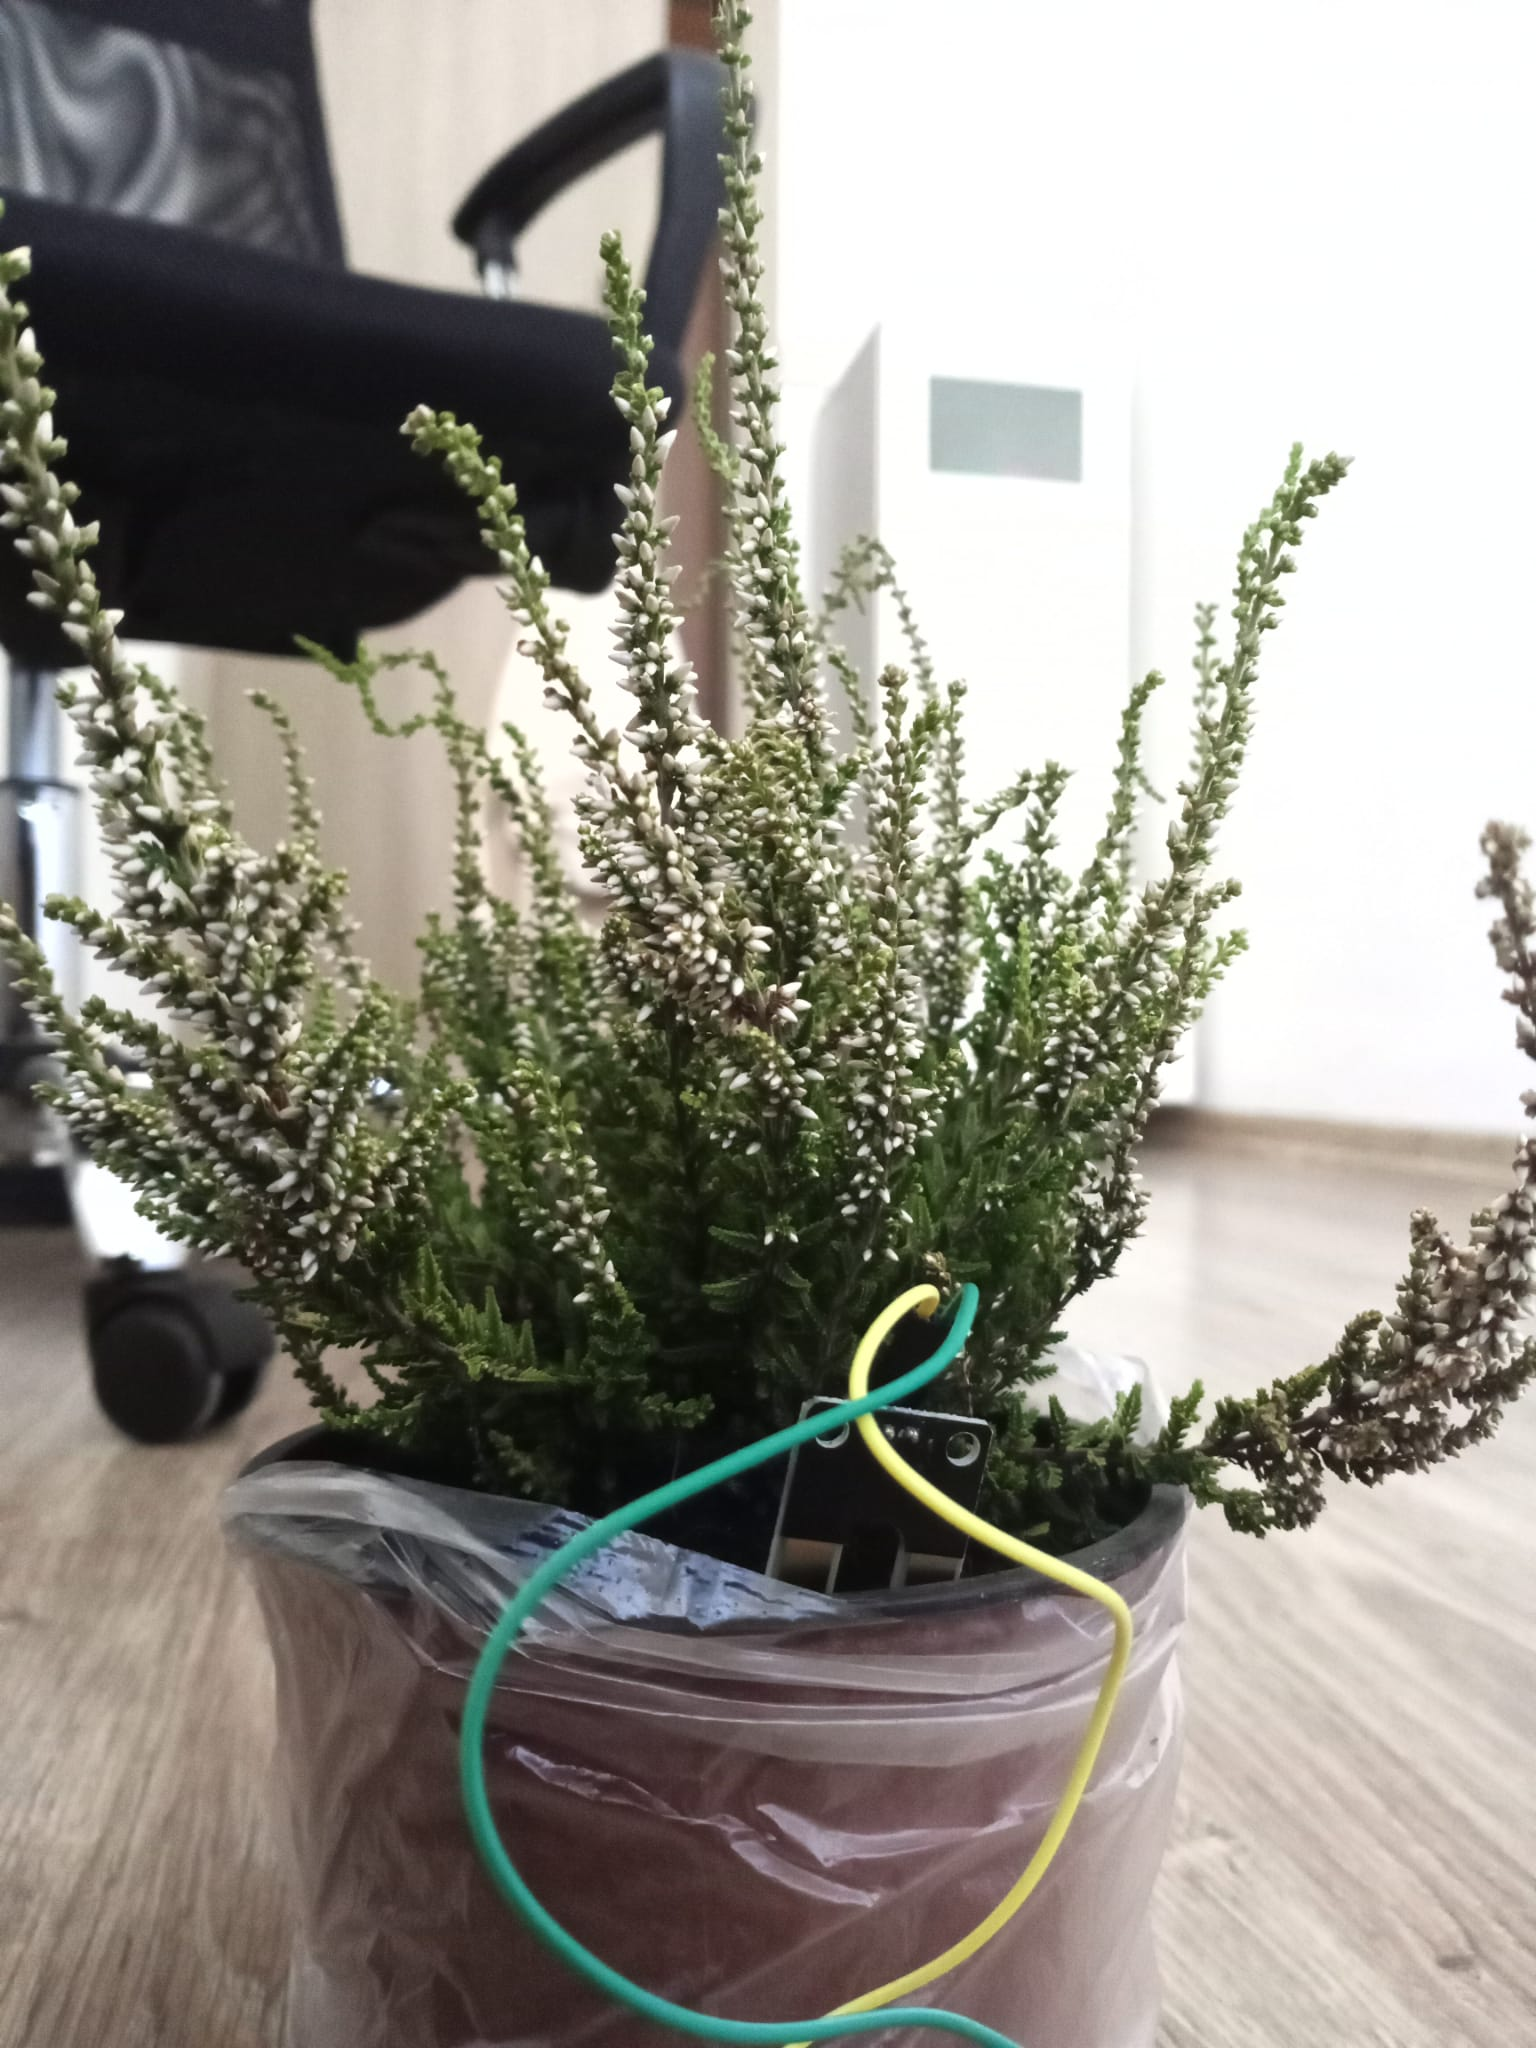
\includegraphics[width=0.4\textwidth]{fig/erica.jpg}
    \caption{Erica with FC-28 sensor}
    \label{fig:erica}
\end{figure}


Installing the hygrometer sensor is trivial, we just need to insert in the soil carefully so the roots of the plant will not get damaged. Now let's start our Arduino program and see what output is printing.

\begin{figure}[H]
    \centering
    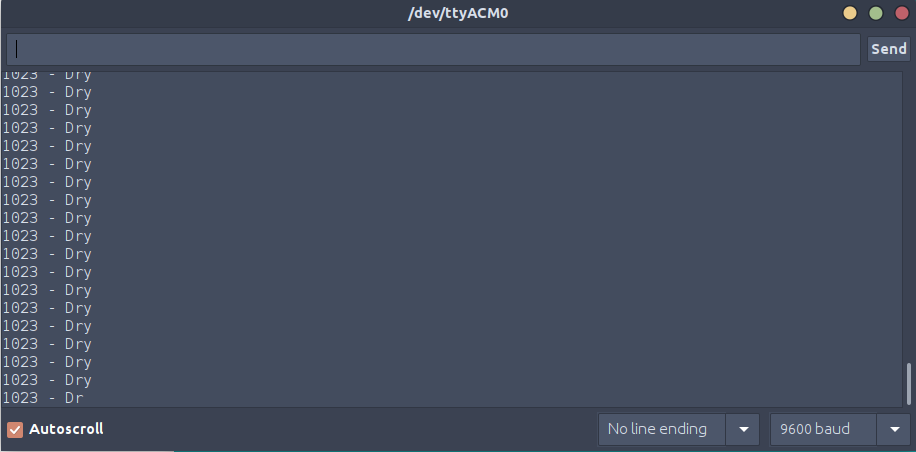
\includegraphics[width=1\textwidth]{fig/seco.png}
    \caption{Arduino output for dry soil}
    \label{fig:dry-soil}
\end{figure}

It is indicating the soil is very dry, as it was to be expected.

\textbf{Second case scenario: watered Erica} \\
Without changing the FC-28 sensor or stopping our current Arduino process, let's water Erica and see how the output changes.

WATERED ERICA

\begin{figure}[H]
    \centering
    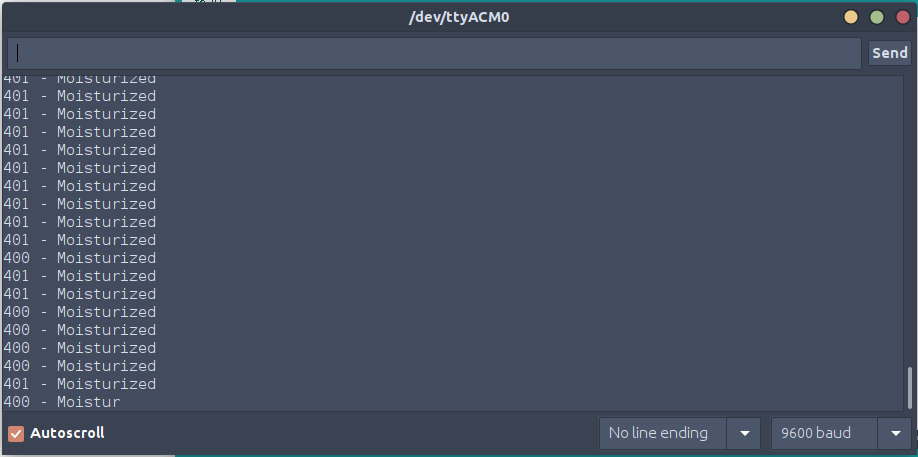
\includegraphics[width=1\textwidth]{fig/humedo.png}
    \caption{Arduino output for humid soil}
    \label{fig:humid-soil}
\end{figure}


As it can be observed, this is quite a simple procedure to check the sensor is behaving as it should, but it is definitely more than enough to server our purpose.

\subsection{Temperature sensor}
The DHT11 sensor\cite{dht11-manual} allows us to measure both temperature and humidity. It consists of an 8-bit microcontroller and two sensors tucked into a tiny blue plastic box. In this section we will see how to measure temperature, in the following section we will focus in measuring humidity.

\begin{figure}[H]
    \centering
    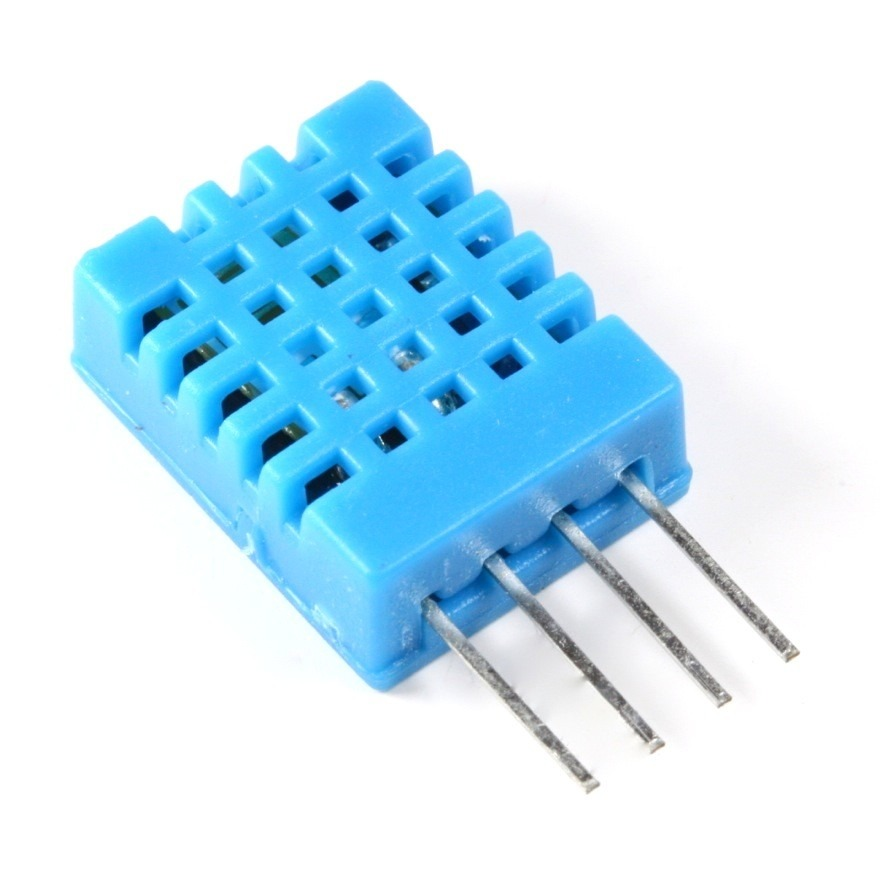
\includegraphics[width=0.3\textwidth]{fig/dht11.jpg}
    \caption{A DHT11 sensor}
    \label{fig:dht11}
\end{figure}

There are many applications for this sensor, it can be implemented as dehumidifier, for automatic control, data loggers or even weather stations. 


\subsection{LDR Sensor}
LDR (which stands for Light Dependent Resistor) sensor is a device used to detect light, it is a resistor made of semiconductor materials. This sensor is really sensitive to light. The stronger the light is, the lower the resistance. There are several uses for this kind of sensor, not only can you measure the value but also turn ON and OFF the light depending on the ambient light intensity.

\begin{figure}[htp]
    \centering
    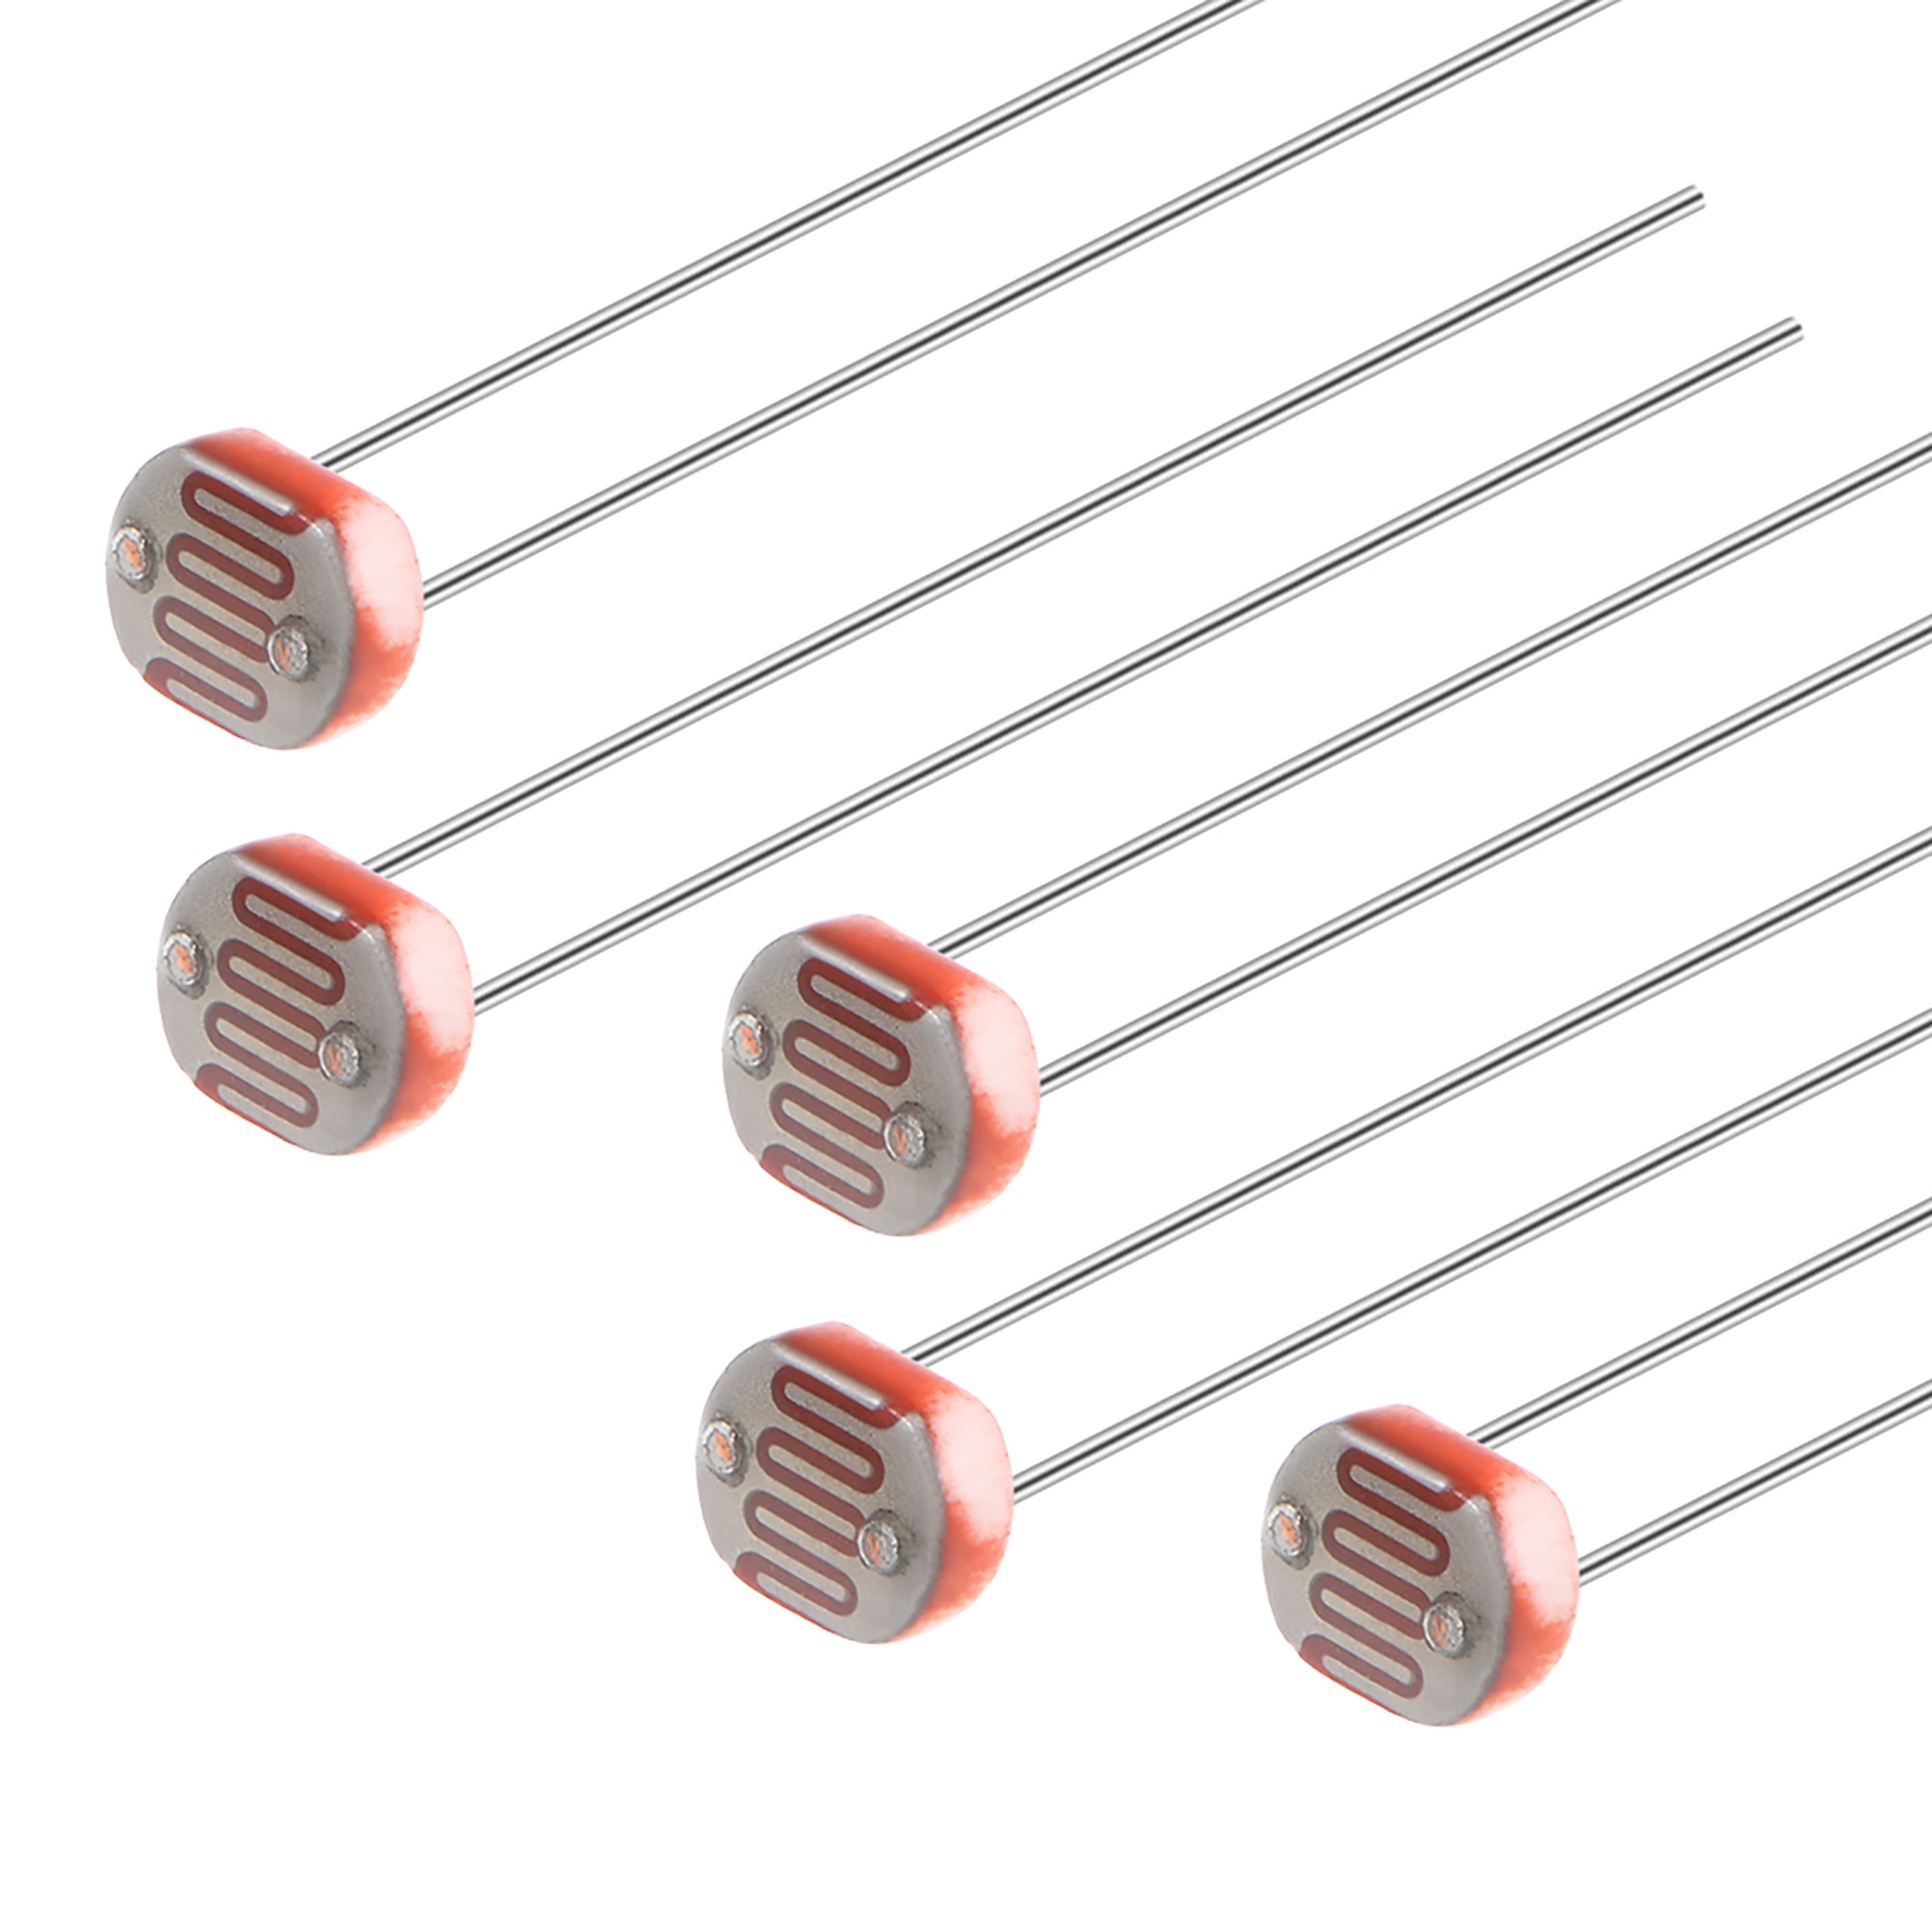
\includegraphics[width=0.35\textwidth]{fig/ldr.jpg}
    \caption{A LDR sensor}
    \label{fig:ldr}
\end{figure}

\subsubsection{Using the sensor}

This is a general view of how the LDR sensor looks connected to the Arduino board in a real life scenario.

\begin{figure}[H]
    \centering
    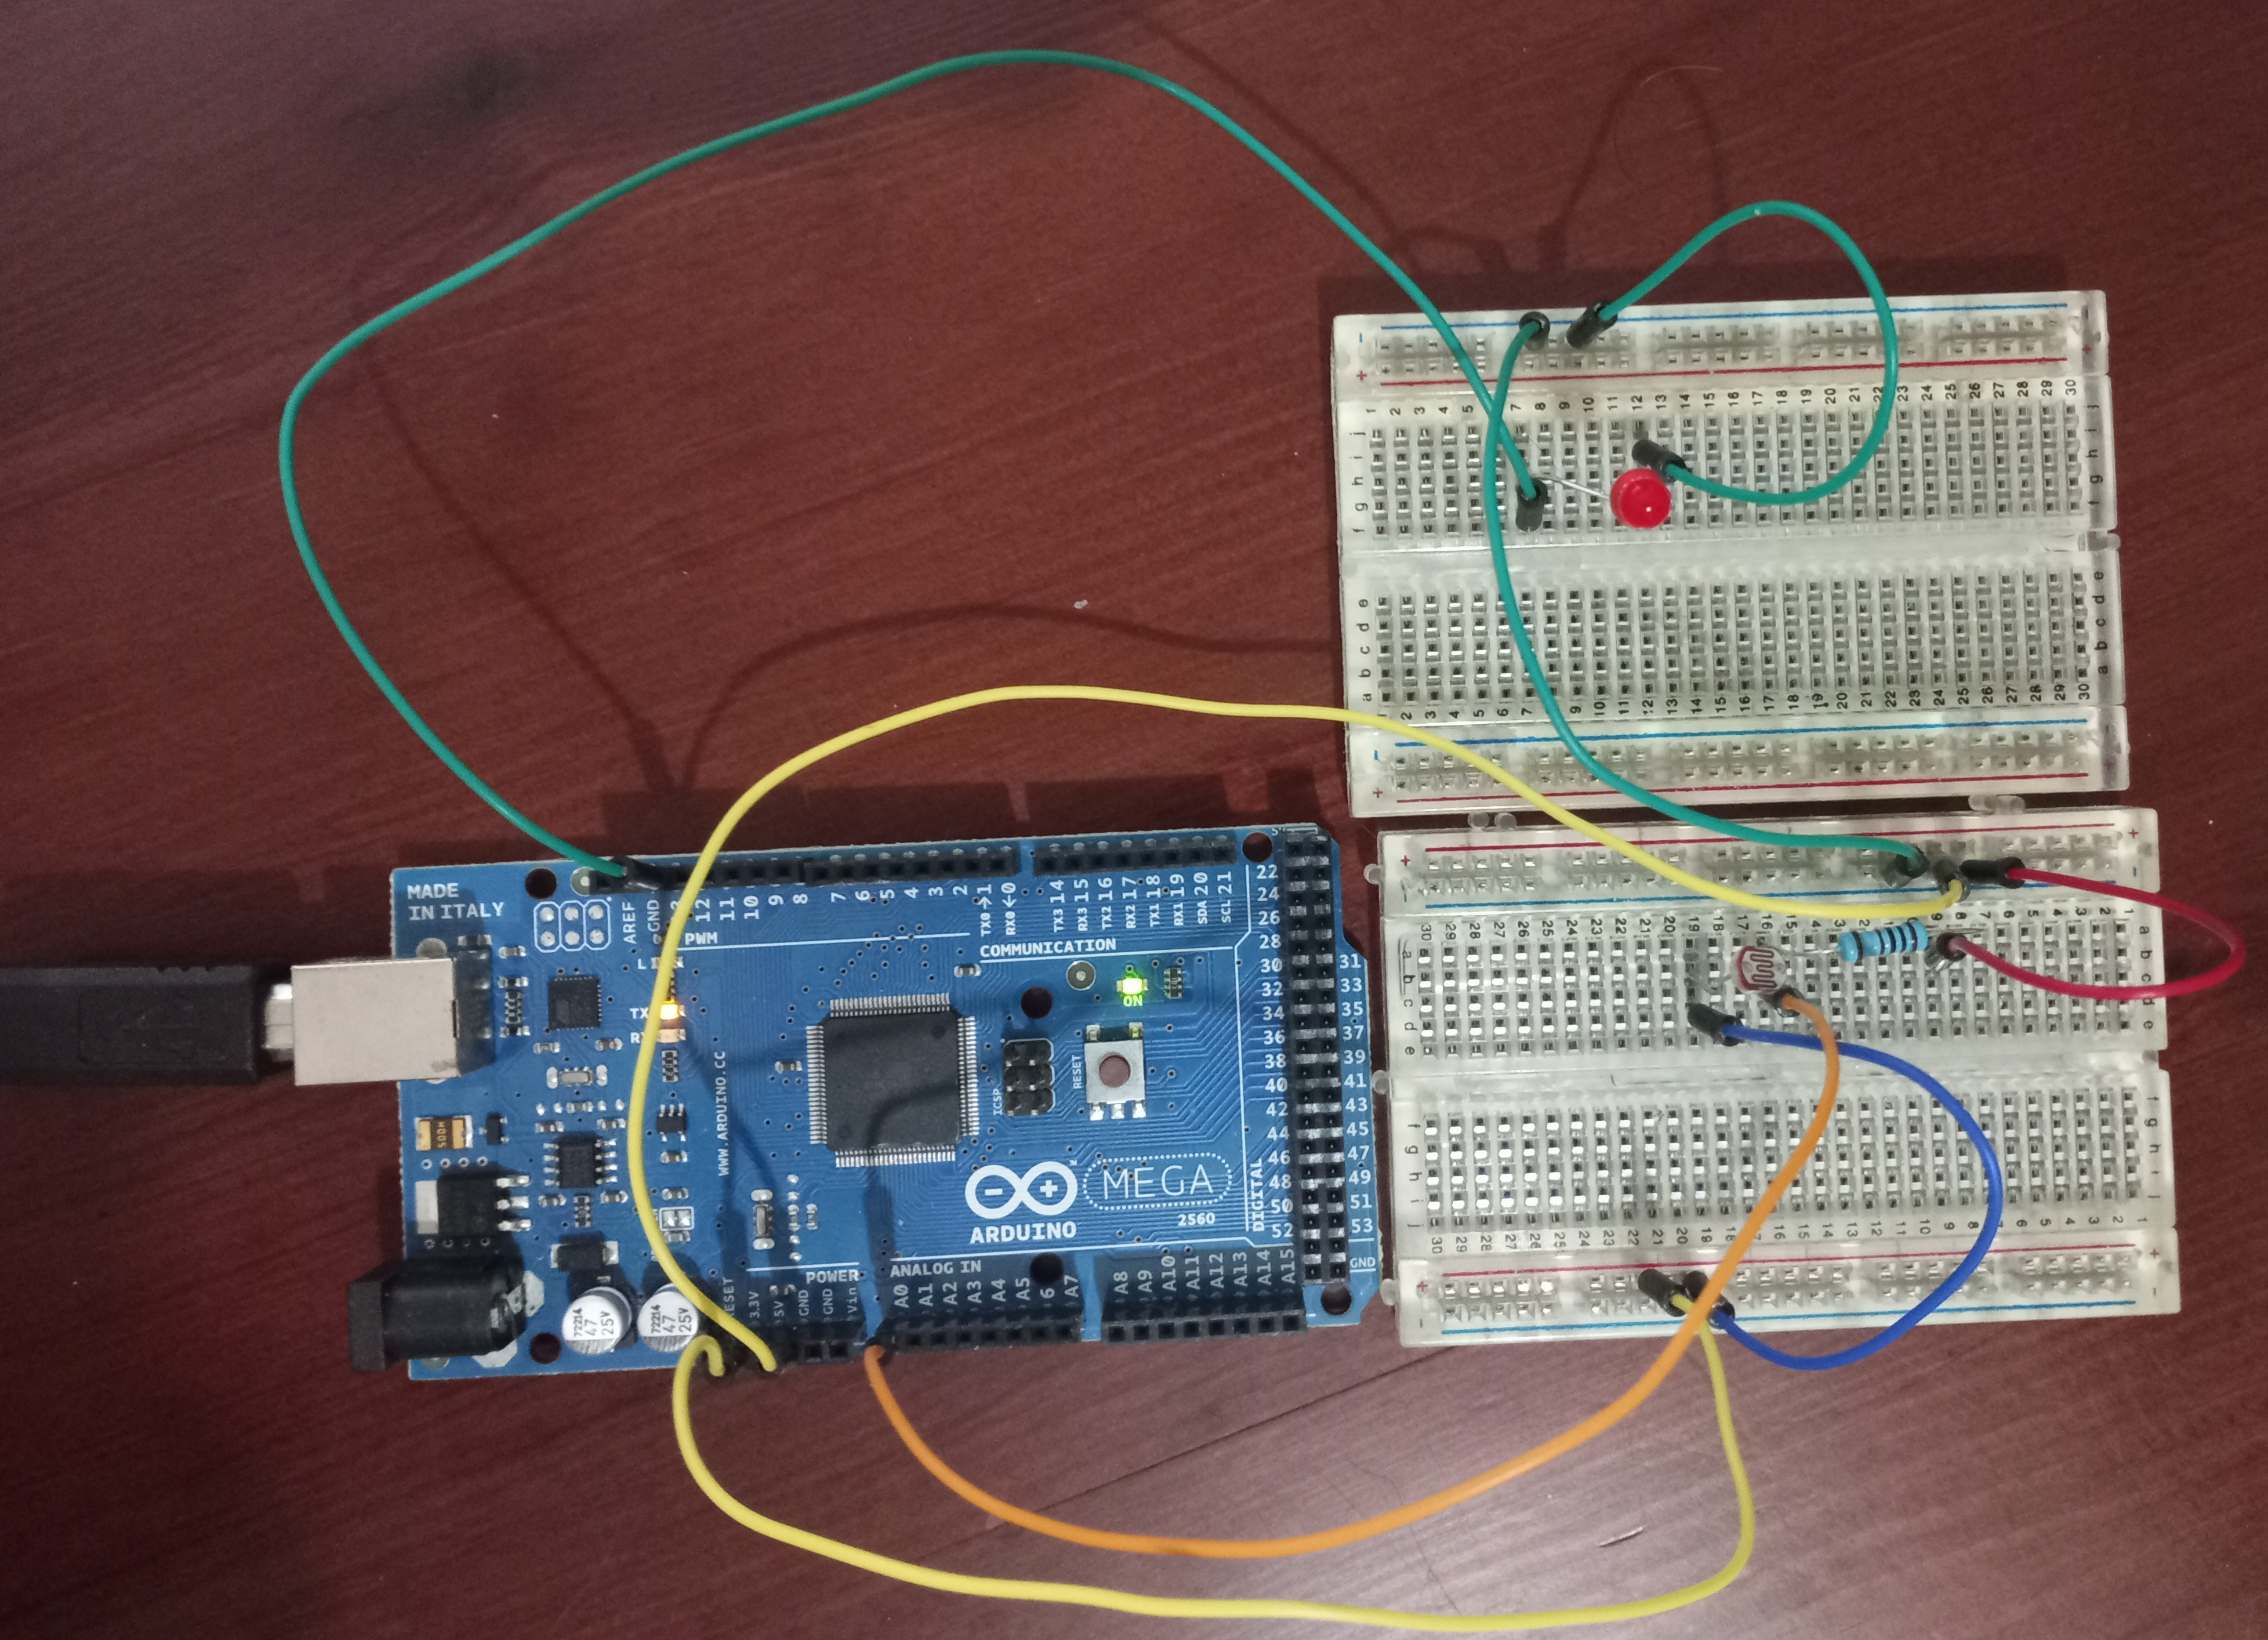
\includegraphics[width=0.5\textwidth]{fig/ldr-circuit.jpg}
    \caption{A LDR sensor}
    \label{fig:ldr}
\end{figure}

Here's a piece of code that will start the sensor and get it to work.
\lstinputlisting{arduino/ldr.ino}

\textbf{LDR code explanation}

In lines 2, 3 and 4 we will initialise the variables we are going to be using for this program.
\begin{itemize}
	\item sensorPin A0 is the input pin that will gather information from the LDR
	\item sensorValue will store the value whatever sensorPin has found coming from the sensor
	\item ledPin will be the output pin connected to the LED
\end{itemize}

In the setup() the ledPin mode will be set as output pin 2.

It gets a bit more interesting in the loop() function. As we did for FC-28, here we are also using analogRead to get the value from sensorPin, for the same reasons that we did in FC-28 too. Then we print the value coming from the sensor as this information might be useful for the user.

In line 14, there is a simple if conditional. A
\begin{figure}[H]
    \centering
    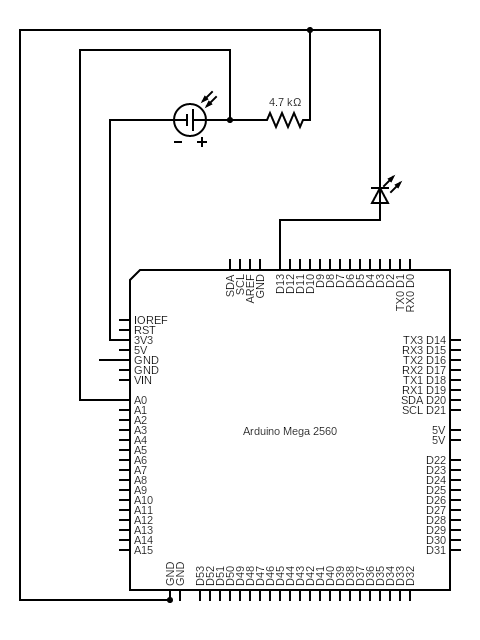
\includegraphics[width=0.7\textwidth]{fig/ldr-scheme-circuit.png}
    \caption{LDR circuit diagram}
    \label{fig:ldr}
\end{figure}


\subsubsection{Testing}

\subsection{PIR Motion sensor}
Another interesting asset that is about to be specified is the passive infrared motion sensor\cite{pir-guide}. In a nutshell, it can detect movement of objects that radiate infrared light, like humans. Because of this, and its eficiency and unexpensiveness, it's a sensor relatively common in security systems and it can have a lot of different applications in farming.

Some applications, besides of course the ones more related to security such as intruder detection, might include automatically switching ON and OFF several devices. See for example turning on a light when movement is detected, so the farmer or worker can forget about lighting and just focus in the main task.

\begin{figure}[H]
    \centering
    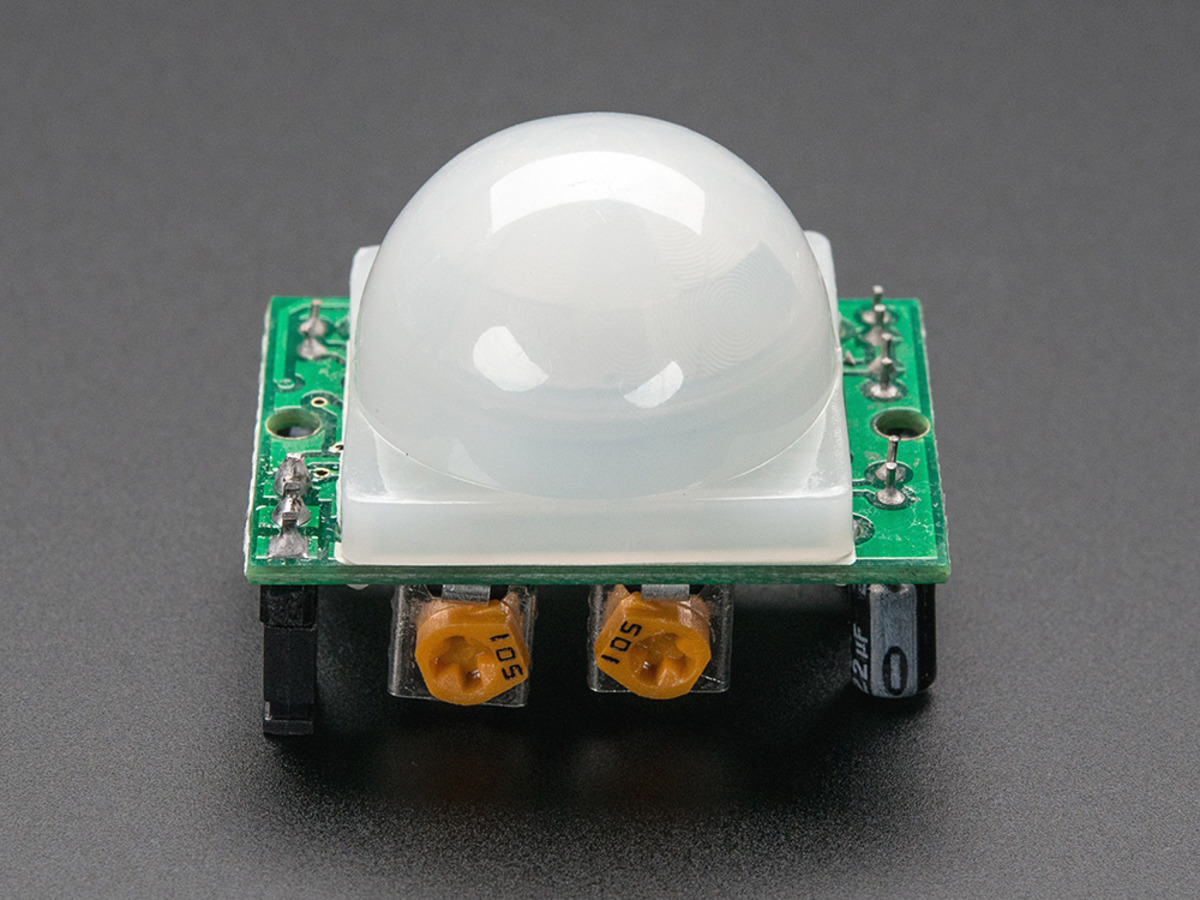
\includegraphics[width=0.35\textwidth]{fig/pir.jpg}
    \caption{Frontal view of PIR motion sensor}
    \label{fig:pir}
\end{figure}


There are several models of PIR motion sensors, but they all work pretty much in the same way. Let's see a bit of that.

They usually have a VCC pin, a GND pin and a digital output. The spherical form of the sensor improves the viewing angle. The PIR output can be connected to any digital pin of our Arduino board, the pin value will be set to "1" is the sensor detects any movement.

This is how a PIR sensor looks like upside down.

\begin{figure}[H]
    \centering
    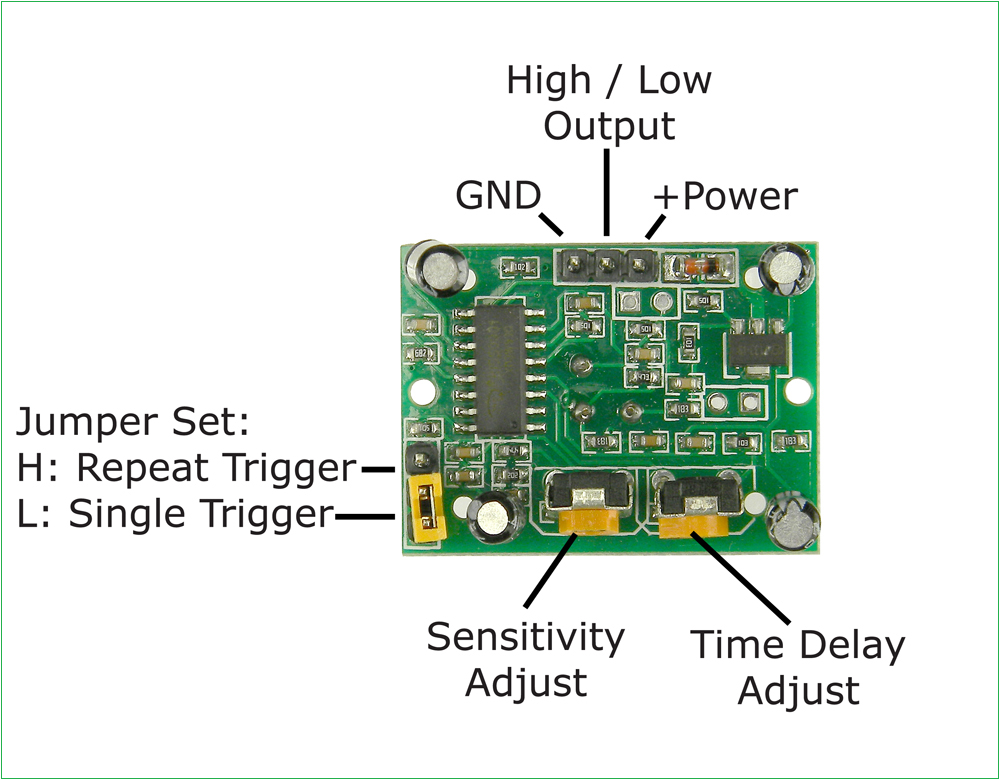
\includegraphics[width=0.6\textwidth]{fig/pir-upside-down.png}
    \caption{Upside down view of PIR motion sensor}
    \label{fig:pir-upsidedown}
\end{figure}

In this image, obtained from the Theory Circuit\cite{theory-circuit} blog, we can spot some parts of the sensor that are worth mentioning:

\begin{itemize}
	\item \textbf{Time Delay Adjust.} How long the output remains set to "1" after detecting motion.
	\item \textbf{Sensitivity Adjust.} Sets the detection range.
	\item \textbf{Single Trigger Mode / Non-repeat Mode(L).} Changes state every time a motion is detected. If we tried it in a practical example, we would see that the LED does not stay on when moving in front of the sensor, but turns on and off every second approximately. This is also called "non-retriggering". 
	\item \textbf{Repeat Trigger Mode(H).} For this position the sensor will turn on every time motion is derected and turn off a bit after the last motion. The way this works is by reseting the timer every single time a motion is detected. This is also called "retriggering". This mode is preferable for most applications, and it is the one we will be using in this project.
\end{itemize}

\subsubsection{Using the sensor}
Now that we have talked a bit about the behaviour of this PIR sensor, let's see how it can be implemented with a really simple example. In order to do so, let's start by taking a look at the circuit.

\begin{figure}[H]
    \centering
    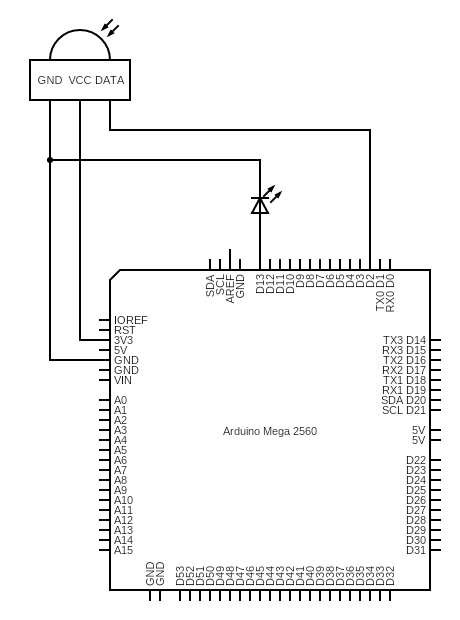
\includegraphics[width=0.7\textwidth]{fig/pir-scheme-circuit.png}
    \caption{Upside down view of PIR motion sensor}
    \label{fig:pir-scheme-circuit}
\end{figure}

In the circuit we have used a LED that will turn on when movement is detected. As it was mentioned before, the PIR is set to retriggering (H mode).

The output of the PIR sensor goes to pin 2 and then the pin 13 is connected to the LED. As it can be easily guessed, the LED pin will be set to OUTPUT mode and PIR pin to INPUT.

Here's a few lines of code for the circuit below.

\lstinputlisting{arduino/pir.ino}

\vspace{5mm}
\textbf{PIR code explanation}

This structure is pretty much the same as what we have seen in the previous code explanations. There is, however, something interesting in line 12 and 16. We have some HIGH and LOW values.

We have not used this values before, le0x1t's use them now. We can take a look at \verb|hardware/arduino/cores/arduino/Arduino.h| file. If we go to lines 18 and 19 of this file we can find the following:
\begin{verbatim}
    18 #define HIGH 0x1
    19 #define LOW  0x0
\end{verbatim}
We can see this are values defined in hexadecimal, if we convert this to decimal, we have 1 and 0 respectively.

Back to the code. If we get a 1 in pirStat then we will get a message saying `Hey! I got you' and it will turn the led on thanks to digitalWrite.

In any other case, we have no movement so the led will be turned off.

\subsection{Ultrasonic sensor}
This ultrasonic distance sensor provides precise, non-contact distance measurements. It works in the same way as bats do: they emit quick and high-frequency sounds pulses, if they hit an object then then the signal comes back to the sensor.

\begin{figure}[H]
    \centering
    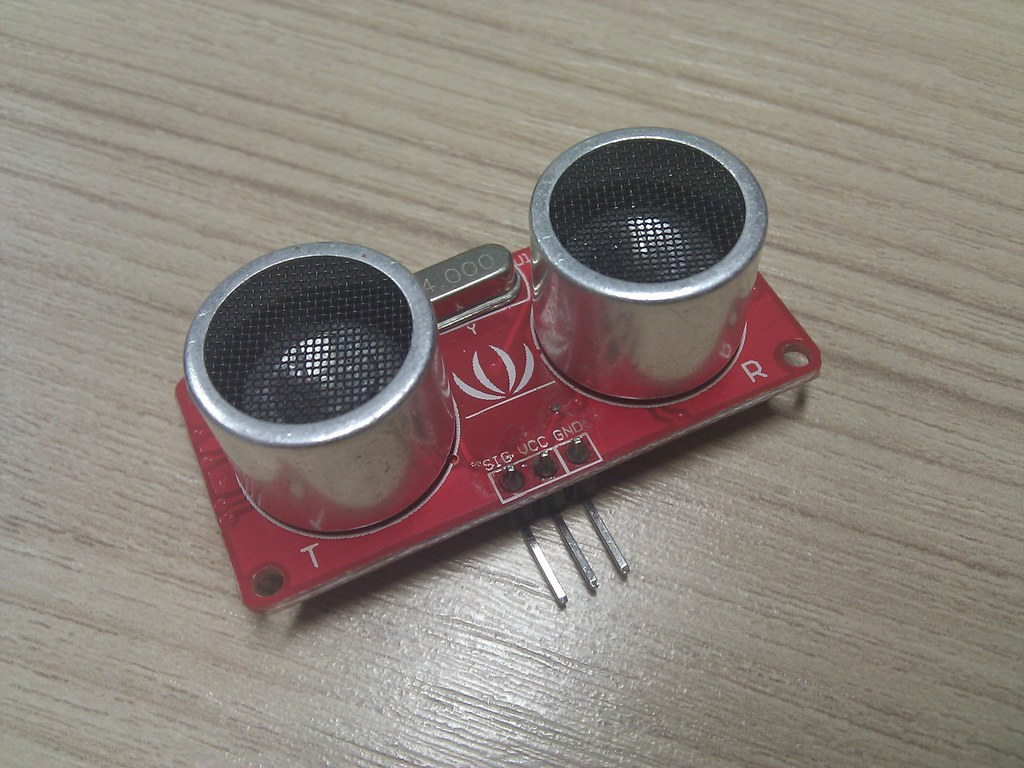
\includegraphics[width=0.55\textwidth]{fig/ultrasonic.jpg}
    \caption{An ultrasonic sensor from Seeedstudio}
    \label{fig:ultrasonic}
\end{figure}

In the previous section, we have seen a PIR sensor. It is interesting to see which are the main differences between these two components that may seem similar but they definitely are not.

	The main difference is the way in which they work: ultrasonic sensors use echolocation\cite{echolocation}, roughly that is the ability to find out the current location using reflected sound, whereas PIR sensors use infrared rays to decide whether there is anyone present.

	Using one or another depends on the needs of the user. If only interested in knowing if there is someone or not, PIR sensor is possibly a better choice. However, if knowing the distance to the object is needed, then we need to use an ultrasonic sensor.

	Notice as well that PIR sensors do not detect intert bodies, that is definitely something to take into account if we are not only interested in detecting humans or animals.

Further, more detailed specifications can be found in the datasheet\cite{ultrasonic-datasheet}
		
\begin{figure}[H]
    \centering
    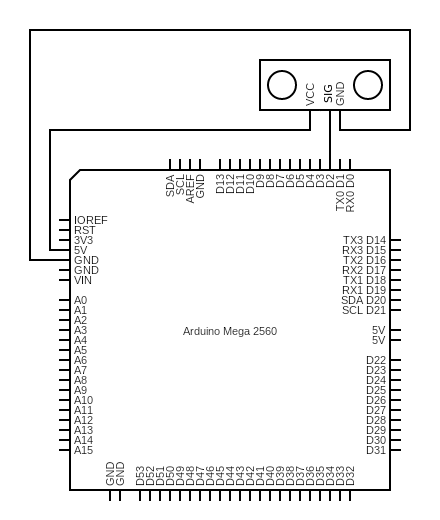
\includegraphics[width=0.7\textwidth]{fig/ultrasonic-scheme-circuit.png}
    \caption{Upside down view of PIR motion sensor}
    \label{fig:ultrasonic-scheme-circuit}
\end{figure}


\lstinputlisting{arduino/ultrasonic.ino}

\textbf{Ultrasonic sensor code explanation}

We are starting this code by defining a variable what will count centimeters, these is of course the distance from the object (or obstacle) being measured to the ultrasonic sensor.



\section{Raspberry Pi server hosting}

\subsection{Introduction}
In this chapter we will walk through the installation and set up of a farmOS system in an Ubuntu Server hosted in a Raspberry Pi.

\subsection{Raspberry Pi configuration}
For our particular case we will be using a Raspberry Pi 4 Model B computer with 2GB RAM. The operating system that will be used is Ubuntu Server 20.

The installation is trivial thanks to the Raspberry Pi Imager, an imaging utility provided by Raspberry in March last year. \href{https://ubuntu.com/tutorials/how-to-install-ubuntu-on-your-raspberry-pi#1-overview}{This} is the tutorial provided by Ubuntu on how to install Ubuntu server in Raspberry Pi using the Raspberry Imager.

After following the tutorial and configuring our Internet connection, we have the Raspberry with Ubuntu server up and running. Since we are using a Spanish keyboard layout, we will also change the main layout
\section{Drupal and farmOS installation}

Testing different environments is objectively tricky. We sometimes do not know the whole configuration, we might encounter problems in some environments that are not appearing in others, etc. That is to say we sometimes do not know how our program is going to behave because of the features of the environment that it is being run in. This is something far from desirable.

This is where Docker plays a role. It allows our program, or in this particular case farmOS, to run isolated from the rest of your machine. It will run in its very own Docker container with everything is needs to correctly be executed to ensure it works seamlessly in any environment. 

\begin{figure}[H]
    \centering
    
\includegraphics[width=0.5\textwidth]{fig/docker_logo.png}
        \caption{Docker}
    \label{fig:docker-logo}
\end{figure}

Docker has a tremendous documentation but we will not be extending any more on this topic, as it is out of the project scope. However, we will elaborate just a bit on docker-compose. As it is the tool we are going to be using to install farmOS.

This is the definition that can be found in the docker docs.

\say{Compose is a tool for defining and running multi-container Docker applications. With Compose, you use a YAML file to configure your application’s services. Then, with a single command, you create and start all the services from your configuration.}

In the same documentation we can also find a well-defined, three-step process to use Compose:
\begin{itemize}
	\item Define your app’s environment with a Dockerfile so it can be reproduced anywhere.
	\item Define the services that make up your app in docker-compose.yml so they can be run together in an isolated environment.
	\item Run docker compose up and the Docker compose command starts and runs your entire app. You can alternatively run docker-compose up using the docker-compose binary.
\end{itemize}

There are some examples as well and a ton of references to useful links, but in simpler words, docker-compose will serve us as a way of managing several containers at once by defining them all in a configuration file. As the reader might have guessed at this point, this is not entirely necesary for us to install and run farmOS, but it is the way the maintainers of the project advise to do it and it also give us scalability that might come in handy in a future.

Since we are speaking about containers, let's just mention Podman before closing this topic. We are not actually going to be using it as farmOS developers use Docker and we want to have our farmOS up and running as soon as possible. However, PODMAN deserves a mention as an alternative to Docker.

The only way of implementing containers is not Docker, there is a whole world beyond. Podman is an open-source tool developed by RedHat. As an advantage, Podman does not use a daemon to manage containers, unlike Docker, which could mean more reliability as it does not depend on a single point. For example, in Docker, if there was a problem with the daemon, we cannot run or manage containers.

Another great pro is that Podman uses exactly the same commands than Docker. Engineers developing the tool did not want to make it confusing so they just used the very same commands. Which means that you could even create an alias docker=podman and start using Podman as if you were using Docker. 

\begin{figure}[H]
    \centering
    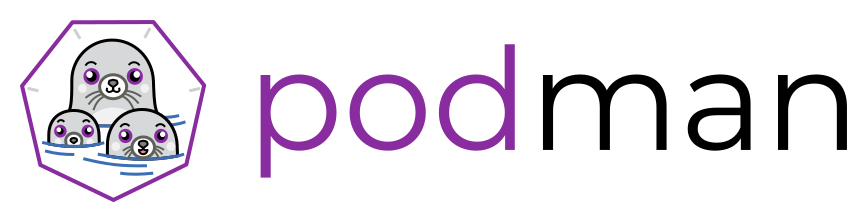
\includegraphics[width=0.5\textwidth]{fig/podman_logo.png}
        \caption{Podman}
    \label{fig:podman-logo}
\end{figure}


Long story short, Podman is, in general terms, more secure than Dockers and offers a few advantages to be taken into account. Again, we are not going to be using it but we considered it was something worthy to be mentioned in this section.

\subsubsection{Getting our hands dirty: farmOS installation}
Without further ado, let's get to it. First step is to go to the documentation of farmOS. The installation is described as a tutorial so we will not spend much time on doing this. Let's follow the tutorial and see if we success. 

This is the \href{https://farmos.org/hosting/docker/}{link}.

Since the tutorial is pretty well defined. We will do a bit of a sum up here in order to understand what's going on during a farmOS installation using Docker.

Honestly, there are many ways to install a Drupal site using Docker. You can browse through dockerhub and just pull the \href{https://hub.docker.com/r/farmos/farmos}{farmOS image} and take a look at the documentation written there. Then, we could run the container and the service will be up.

However, for this project, we will be using docker-compose as Drupal requires a database, it is pretty useful to dockerize both services.

These are the steps I followed to install my farmOS.
\begin{itemize}
    \item Go to the \href{https://github.com/farmOS/farmOS}{farmOS official repository}.
    \item Make sure that you are in the correct version. Although there is a version 2 that has just been released, we are interested in version 7.x-1.x. We will talk about version 2 a bit further.
    \item Clone the repository in your local machine using Git (git clone https://github.com/farmOS/farmOS).
    \item Go to docker directory and copy the file docker-compose.development.yml to docker-compose.yml. The simplest way to do so is by using the terminal. cp docker-compose.development.yml docker-compose.yml.
    \item You are all set. Execute docker-compose up.
\end{itemize}

\textbf{Troubleshooting.} Some errors I usually find every now and then is the ports being used by other service. This is something fairly common if you are used to managing several docker services at once. For a quick fix, just go to our brand-new docker-composer.yml and change the ports defined there.

Now we can open our favourite browser and access localhost. There it is, a nice farmOS instance up and running.

foto farmos

This is a generic Drupal installation screen. Let's install it.

We need to be careful when configuring the database. If the data introduced is not correct, we will be gettings errors and the installer won't let us continue with the installation process.
The data that needs to be introduced in the database is the one appearing in the docker-compose.yml file. Also here's a link with some more information about \href{https://farmos.org/development/docker/}{developing farmOS with docker}, it might come in handy during the completition of the procedure.
 + fotos d la instalación



Let's pull the image by running \verb|docker pull farmos/farmos|.
\begin{figure}[H]
    \centering
    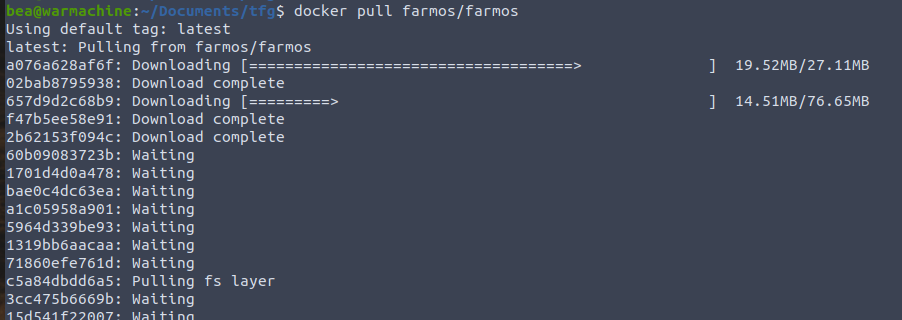
\includegraphics[width=1\textwidth]{fig/pull-docker.png}
    \caption{Docker daemon downloading the farmOS image from dockerhub}
    \label{fig:pull-docker}
\end{figure}

That's done. If you are following my steps you should have something similar to:
\verb|Status: Downloaded newer image for farmos/farmos:latest|



\verb|docker.io/farmos/farmos:latest|

Now let's check the images to make sure farmOS is among them by running \verb|docker images|. Although actually... If like me, you have tons of images downloaded, you can run \verb|docker images | grep "farmos"|.

Next step is to run the container. Let's execute docker run -itd farmos/farmos /bin/bash. and we'll get a container id, which can be useful to identify the container. This is ours: 0541bc7d2dcfe16553ef0364b26239f3d9e7eceacc28dd7c3a99381a65d068ad

Okay, let's list the containers and check if farmOS container is there.

bea@warmachine:~/Documents/tfg$ docker container ls
CONTAINER ID   IMAGE                               COMMAND                  CREATED              STATUS                PORTS     NAMES
0541bc7d2dcf   farmos/farmos                       "docker-entrypoint.s…"   About a minute ago   Up About a minute     80/tcp    affectionate_shannon
58f9af3bc507   drud/ddev-ssh-agent:v1.17.0-built   "/entry.sh ssh-agent"    4 days ago           Up 4 days (healthy)             ddev-ssh-agent

Well. Indeed it is.






\section{Arduino and server communication}
Let's jump in into a really interesting section. How can we establish a communication between our Arduino board, that is collecting sensor data, and the server we just built?

Well, luckily for us, there is quite an useful module called Arduino Ethernet Shield that will connect our board to the Internet in no time.

\subsection{Ethernet shield}
This device that you can see in the picture below connects to the internet using a RJ45 cable, which is basically the regular Ethernet cable we are totally used to seeing pretty much everywhere.

\begin{figure}[H]
    \centering
    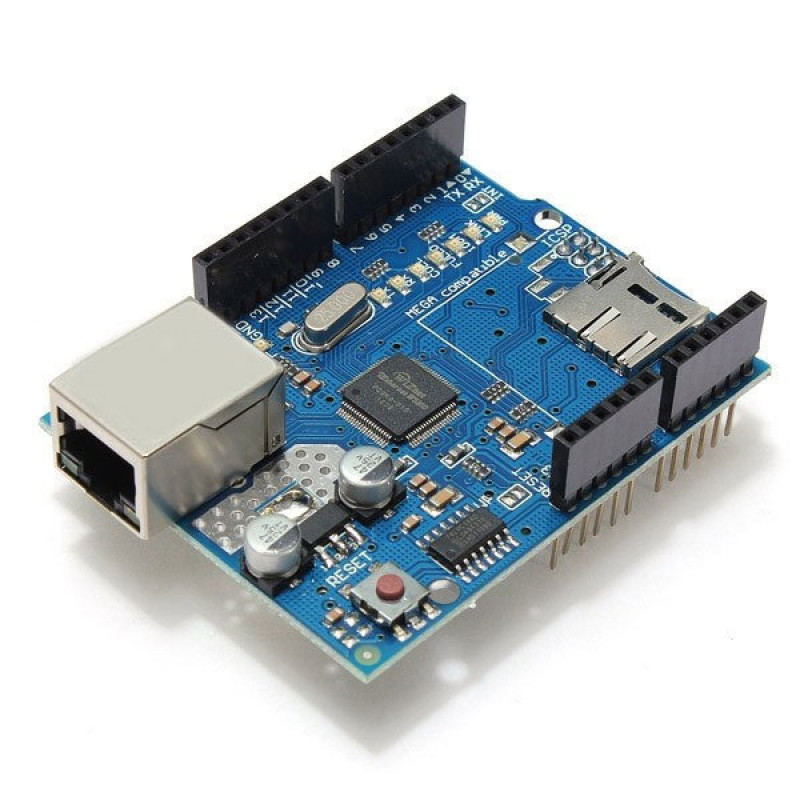
\includegraphics[width=0.5\textwidth]{fig/ethernet.jpg}
    \caption{Arduino Ethernet Shield}
    \label{fig:ethernet}
\end{figure}

\subsubsection{Connecting to the Internet}
Let's start by the beginning, we need to be able to connect to the Internet. This will assure as well that our Arduino is working properly, as well as the Ethernet shield.

The first step is to assemble the Arduino and the Ethernet shield together. We need to make sure that the two ICSPs (In Circuit Serial Programming) are connected. See a picture of the prototype for this project below.

\begin{figure}[H]
    \centering
    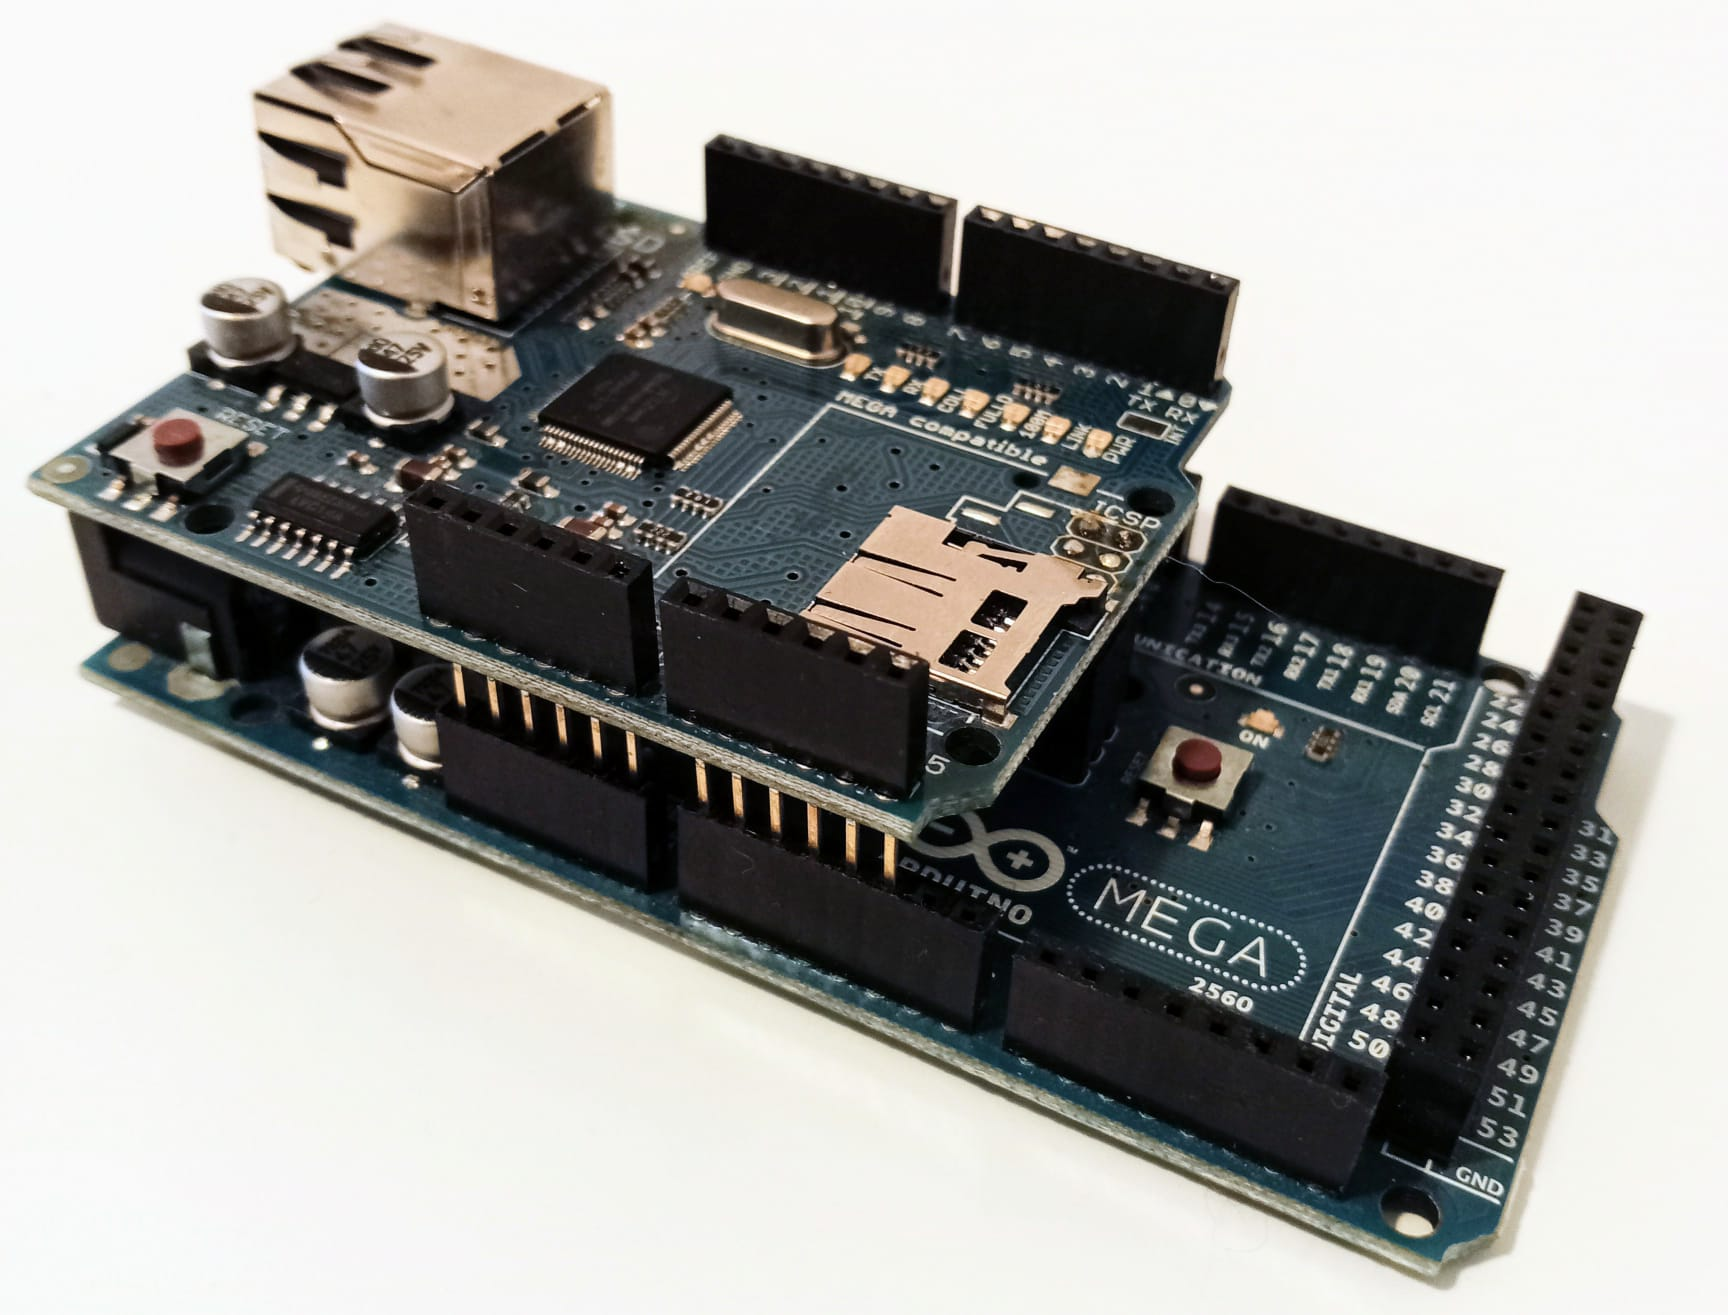
\includegraphics[width=0.7\textwidth]{fig/ethernet-connected.jpg}
    \caption{Ethernet Shield connected to Arduino MEGA 2560}
    \label{fig:ethernet-connected}
\end{figure}

\vspace{7mm}

\textbf{Getting an IP address}

There is a very convenient tool in Arduino IDE that has some example scripts, these are really useful to test simple features without spending too much time.

The example script we are interested in for this particular scenario is the DhcpAddressPrinter sketch. It can be found in \verb|File > Examples > Ethernet > DhcpAddressPrinter| and it looks like this.

\vspace{5mm}

\lstinputlisting{arduino/DhcpAddressPrinter.ino}

\vspace{7mm}

After connecting our Ethernet shield to the RJ45 cable and obviously, the board to the power supply, we will execute this script and see what we get. Here we go.

\begin{figure}[H]
    \centering
    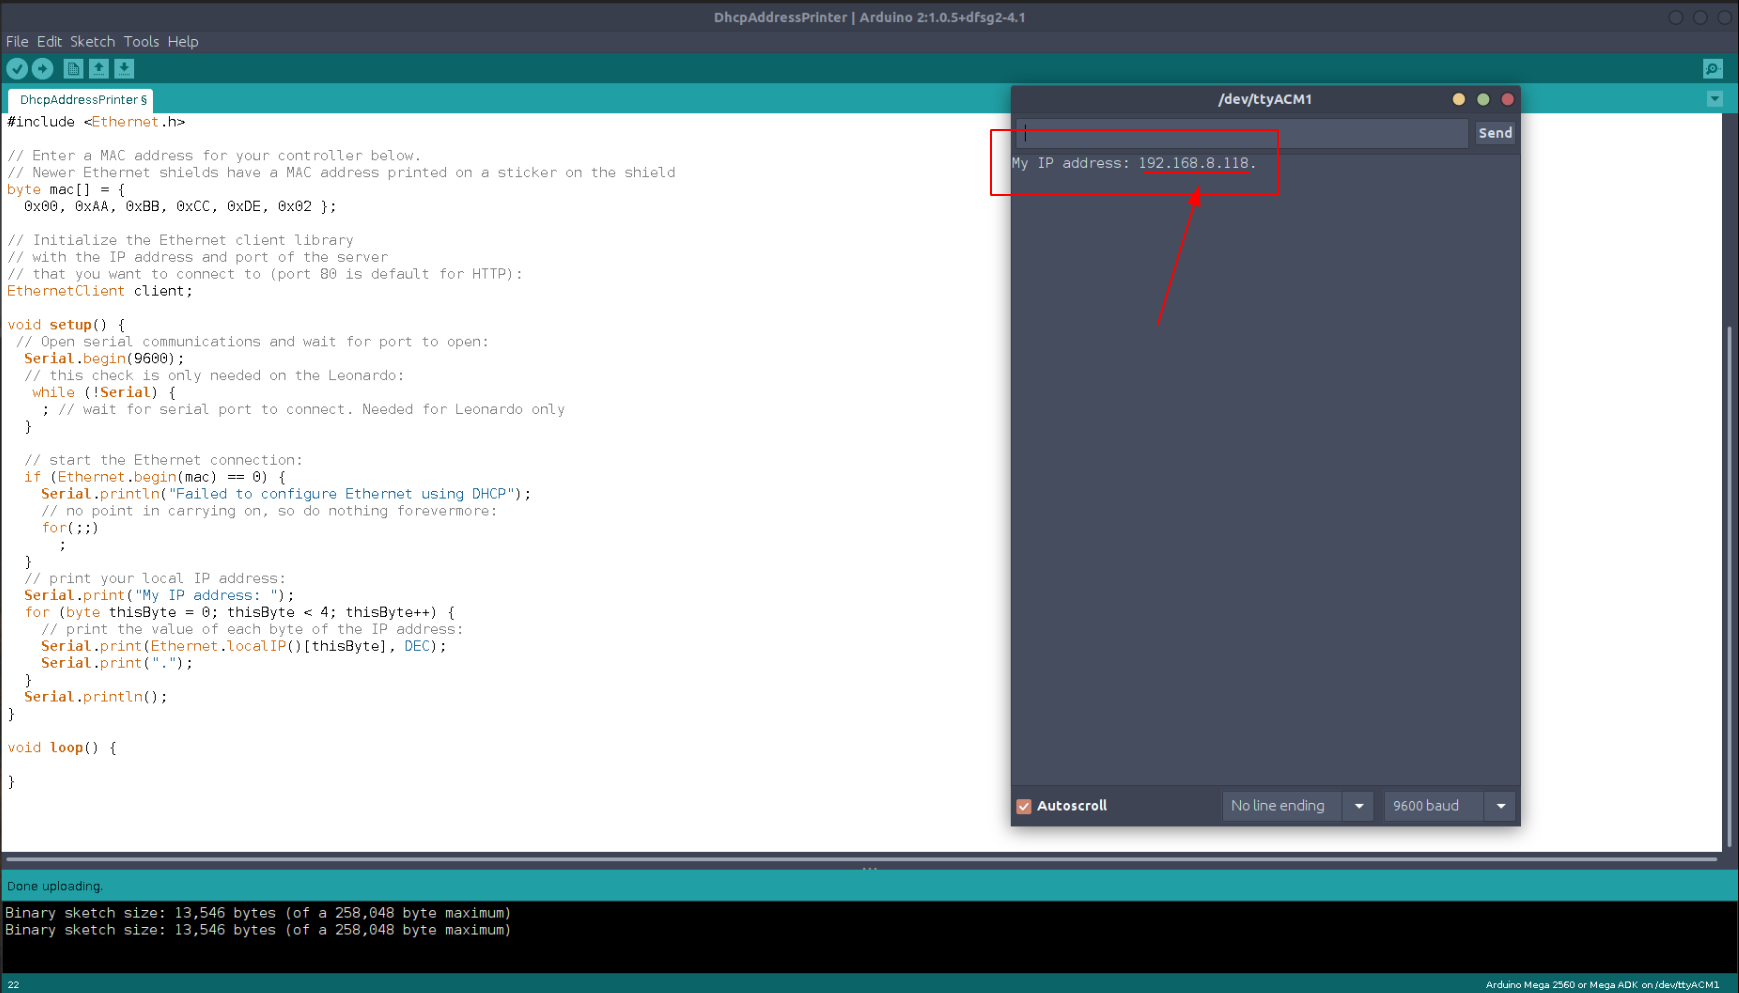
\includegraphics[width=1\textwidth]{fig/assign-ip.png}
    \caption{View of Arduino IDE}
    \label{fig:assign-ip}
\end{figure}

That is a general view of the Arduino IDE executing the \verb|DhcpAddressPrinter.ino| script. Let's take a closer look to the serial monitor, so we can actually read the IP that has been assigned to the device in this moment.

\begin{figure}[H]
    \centering
    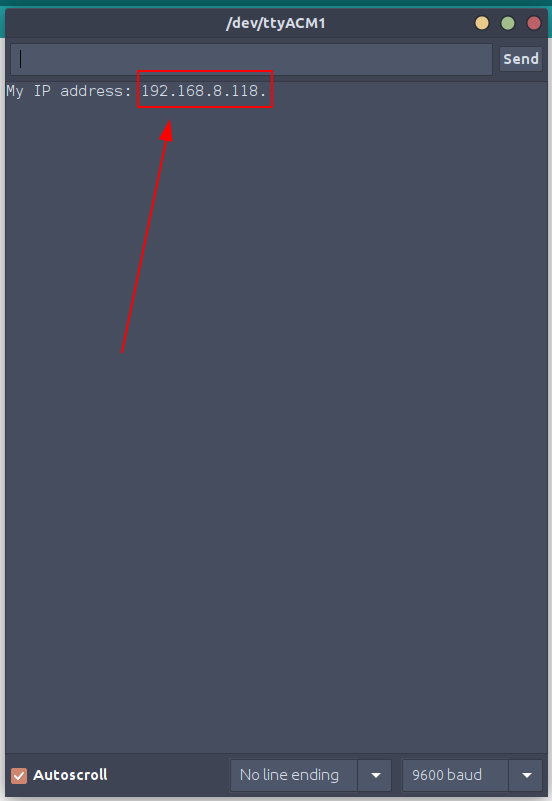
\includegraphics[width=0.7\textwidth]{fig/serial-monitor-ip.png}
    \caption{View of the serial monitor}
    \label{fig:serial-monitor-ip}
\end{figure}

There it is. The current IP address is \verb|192.168.8.118|.

The next step is to write a script so that we can send information, that is make our Arduino device a client and establish a cliente-server communication between the Arduino board and the server hosted on the Raspberry.



\section{Conclusions}


